\documentclass{article}
\usepackage[utf8]{inputenc}
\usepackage[margin=1in]{geometry}
\usepackage[colorlinks]{hyperref}
\usepackage{graphicx}
\usepackage{caption}
\usepackage{color}
\usepackage{subcaption}
\usepackage{float}
\makeatletter
\renewcommand\paragraph{\@startsection{paragraph}{4}{\z@}%
            {-2.5ex\@plus -1ex \@minus -.25ex}%
            {1.25ex \@plus .25ex}%
            {\normalfont\normalsize\bfseries}}
\makeatother
\setcounter{secnumdepth}{4} % how many sectioning levels to assign numbers to
\setcounter{tocdepth}{4}    % how many sectioning levels to show in ToC
\begin{document}
\title{\textbf{CS6011: Kernel Methods for Pattern Analysis}
\\
\textbf{Programming Assignment 1}
}
\author{Aravind Sankar CS11B033 \\
Ramnandan SK CS11B061 \\
Adit Krishnan CS11B063 \\[0.2in]
Group 2
}
\floatplacement{figure}{H}
\maketitle
\tableofcontents 
\newpage
\section{Objective of the assignment}
The basic goal of this assignment is to explore the use of Bayes classifiers, Perceptron and Multi Layer Feed Forward Neural Networks (MLFFNN) for the task of classification, and the use of MLFFNN and Radial Basis Function Neural Networks (RBFNN) for the task of regression.

\section{Classification task}
\subsection{Dataset 1}

\subsubsection{Linearly Separable Dataset}


\subsubsection{Non-linearly Separable Dataset}

\subsubsection{Overlapping classes Dataset}


\subsection{Dataset 2 - Image dataset}



\section{Regression task}

\subsection{Dataset 1 (Univariate)}


\subsection{Dataset 2 (Bivariate)}




%\begin{figure}[H]
%
%\begin{subfigure}{.5\textwidth}
%\centering
%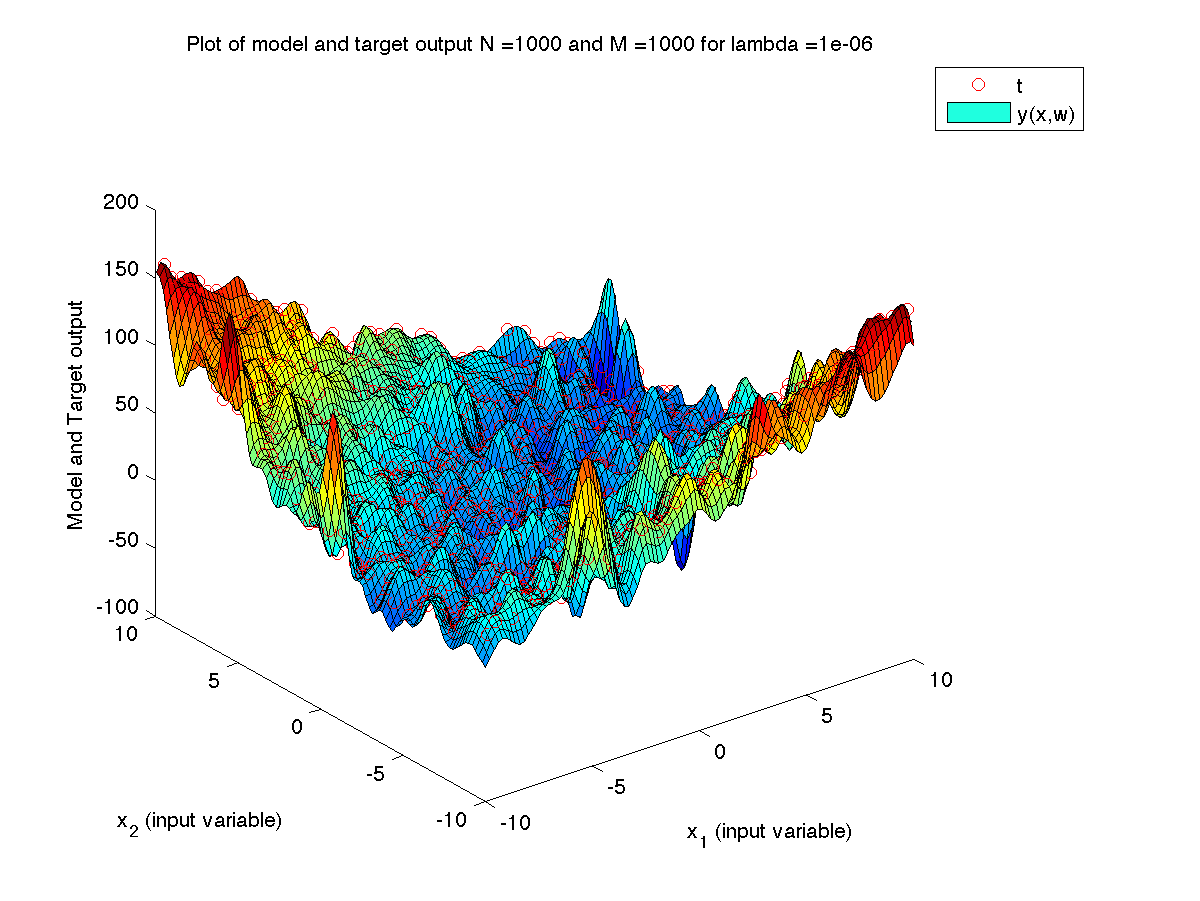
\includegraphics[width=\linewidth]{D2/Varyinglambda_N1000M1000lambda1e-06}
%\caption{$\lambda$ = $10^{-6}$}
%\end{subfigure}
%\begin{subfigure}{.5\textwidth}
%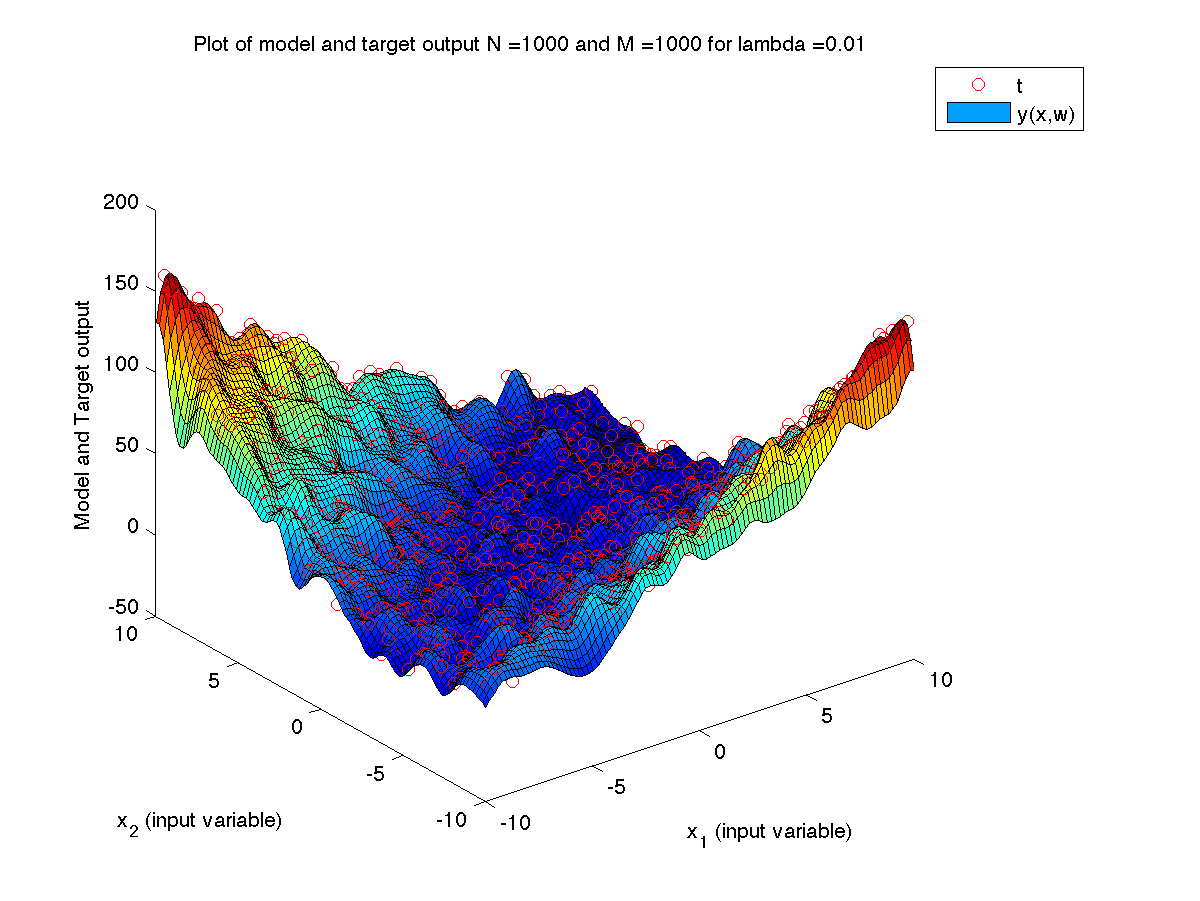
\includegraphics[width=\linewidth]{D2/Varyinglambda_N1000M1000lambda0_01}
%\caption{$\lambda$ = 0.01}
%\end{subfigure}
%
%\end{figure}



\end{document}
